\section{Novel Results}
We continue to extend the rSLDS model using BBVI and Laplace EM inference to dynamical systems exhibiting bifurcations. We wish to see how well the model can recapture the changing dynamics of a fixed point near the bifurcation. First, we examine the Van der Pol oscillator which has a Hopf bifurcation at the origin. Next, we explore the normal form of the Bautin bifurcation which has a bifurcation at the origin.  
% We continue to look at the R\"ossler attractor which has a period-doubling bifurcation. 

\subsection{Van der Pol Oscillator}
The Van der Pol oscillator is a second-order differential equation of the form
\[
    \frac{\ddd^2 x}{\ddd t^2} - \mu(1 - x^2)\frac{\ddd x}{\ddd t} + x = 0,
\]
where $x$ is the spatial coordinates and $\mu$ is a scalar parameter. The equation can be rewritten into its two-dimensional form using the transformation $y = x_t$ to get
\[
    \begin{cases}
        x_t = y,\\
        y_t = \mu(1-x^2)y - x.
    \end{cases}
\]
Setting $x_t$ and $y_t$ equal to zero, we find that the Van der Pol oscillator has a fixed point at the origin $(x,y) = (0,0)$ which is known to have a Hopf bifurcation. This means that the stability of the fixed point is stable for $\mu < 0$ and there are no limit cycles near the fixed point. When $\mu = 0$, the Van der Pol system becomes linear and the origin is a circular node. Lastly, when $\mu > 0$, the fixed point becomes unstable and a stable limit cycle around the origin appears. We demonstrate the different behaviors in Figure \ref{trueVDP}. On the left $\mu > 0$, the stable limit cycle around the fixed point can be seen. In the middle $\mu =0$, the trajectory forms a circle around the center node. On the right $\mu > 0$, the trajectory spirals into the stable fixed point. 

\begin{figure}
    \centering
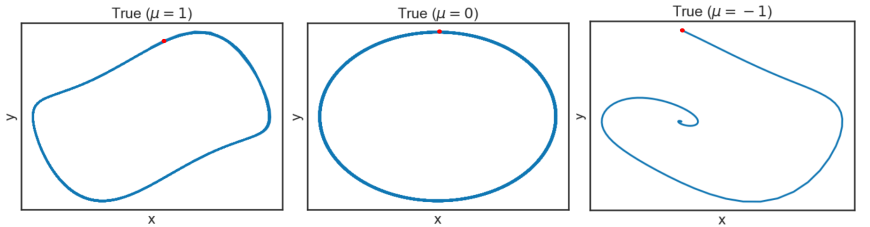
\includegraphics[width=0.90\textwidth,height=\textwidth,keepaspectratio]{./figures/paper_fig10.png}
    \caption{True trajectories of the Van der Pol oscillator used to fit rSLDS model over $T\in[0,1000]$ with $1000$ observations. The initial condition of $(0,2.2)$ can be seen in red. On the left, $\mu =1$ and the stable limit cycle can be seen. In the middle, $\mu = 0$ and the fixed point is a center. On the right, $\mu = -1$ and the fixed point is stable.}
    \label{trueVDP}
\end{figure}

To fit the Van der Pol oscillator to the rSLDS model, we use an ODE solver to generate data from the Lorenz system at a fixed initial condition $(x,y) = (0,2)$ and $t \in [0,1000]$ using $10000$ observations. To study how the model handles bifurcations, we sample the trajectory when $\mu = -1,0,1$ which are around and on the bifurcation. The true trajectories that are used to train the model can be seen in Figure \ref{trueVDP}. Once again, we enhance the realism of our data by adding Gaussian noise. In the $\mu = 1$ case, we expect a stable limit cycle that has two prominent states and thus we construct the model using two discrete states. For the sake of consistency, we set the model to have two discrete states for each $\mu$ value. 



By fitting and training an rSLDS model for each $\mu$ value using the BBVI and Laplace EM methods, we recover the trajectories of the original system which are presented in Figure \ref{badvdp}. While the rSLDS model was able to recover the trajectories for the $\mu=0,1$ case, the model failed to rediscover the behavior at $\mu = -1$. To handle this, we turn down the amount of Gaussian noise being added to the observations. Retraining the model we recover the dynamics of the $\mu = -1$ as seen in Figure \ref{goodvdp}. When comparing the results to the true trajectories, we see that for each $\mu$ value, the rSLDS models using Laplace EM and BBVI are both able to accurately recover the behavior of the Van der Pol system near the bifurcation. When $\mu = 1$, both models identify two latent states exceptionally well. In the $\mu = 0$ case, although the BBVI method struggles to identify the latent states by overlapping the latent states, the Laplace EM model identifies one latent state for the entire trajectory. On the other hand, when $\mu = -1$ both methods struggle to identify the latent states.
\begin{figure}
    \begin{subfigure}[b]{0.33\linewidth}
        \centering
        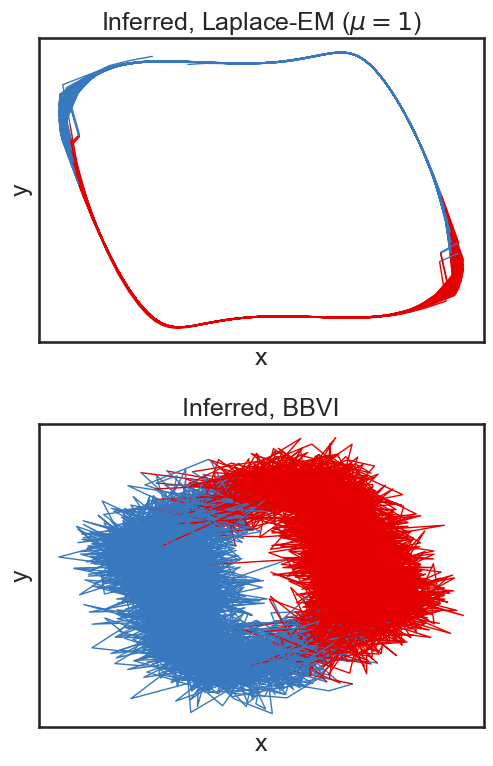
\includegraphics[width=\linewidth]{./Figures/vdp-bad-mu1.png}
        \caption{}
        \label{badvdp:a}
        \vspace{4ex}
    \end{subfigure}%%
    \begin{subfigure}[b]{0.33\linewidth}
        \centering
        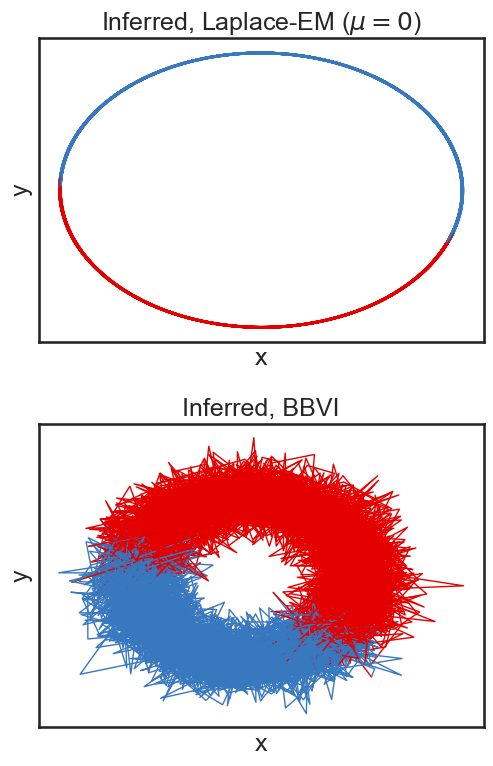
\includegraphics[width=\linewidth]{./Figures/vdp-bad-mu0.png}
        \caption{}
        \label{badvdp:b}
        \vspace{4ex}
    \end{subfigure}%%
    \begin{subfigure}[b]{0.33\linewidth}
        \centering
        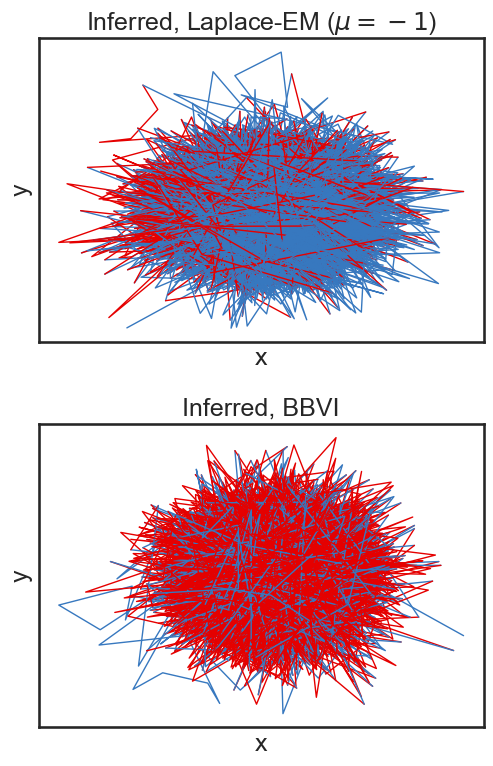
\includegraphics[width=\linewidth]{./Figures/vdp-bad-mu-1.png}
        \caption{}
        \label{badvdp:c}
        \vspace{4ex}
    \end{subfigure}
    \caption{Recovered trajectories of the Van der Pol oscillator from rSLDS model using the Laplace-EM and BBVI methods with Gaussian noise present. In (A), $\mu = 1$ and the Laplace-EM recovers the system with two latent states, seen in blue and red, but BBVI has a high amount of noise. In (B), $\mu = 0$ and the same results occur as in (A). In (C), $\mu = -1$ and both methods fail to recover the true behavior.}
    \label{badvdp}
\end{figure}


\subsection{Bautin Bifurcation}
We extend our examination of bifurcations to see how the models handle a generalized Hopf bifurcation. Consider the autonomous system of ordinary differential equations
\[
    \dot{y} = f\paren{y, \beta},
\]
where $y = (y_1,y_2)^T \in \R^2$ are the spatial coordinates and the system depends upon $\beta = (\beta_1,\beta_2) \in \R^2$. Supposing the system has a fixed point on the origin, the fixed point is said to experience a generalized Hopf bifurcation known as a Bautin bifurcation if specific conditions upon the first and second Lypanonuv coefficients, the details are omitted as they are not deemed insightful to the paper. When these conditions are met, $\dot{y}$ is locally equivalent near the origin to 
\[
    \begin{cases}
        \dot{y_1} = \beta_1 y_1 - y + \beta_2 y_1 \paren{y_1^2 + y^2} + \sigma y_1 \paren{y_1^2 + y^2}^2,\\
        \dot{y_2} = y_1 + \beta_1 y + \beta_2 y \paren{y_1^2 + y^2} + \sigma y \paren{y_1^2 + y^2}^2,
    \end{cases}
\]
which is the normal form of the Bautin bifurcation. Here $\sigma = \pm 1$ is related to the sign of the first Lypanonuv coefficient. 

\begin{figure}
    \begin{subfigure}[b]{0.33\linewidth}
        \centering
        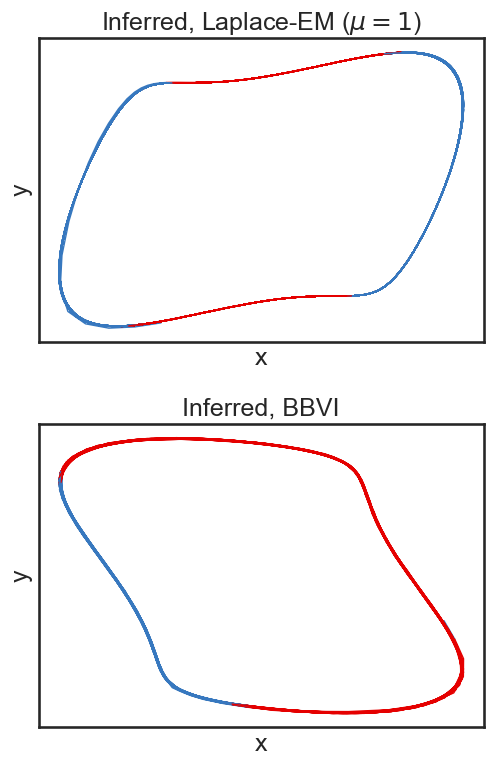
\includegraphics[width=\linewidth]{./Figures/vdp-good-mu1.png}
        \caption{}
        \label{goodvdp:a}
        \vspace{4ex}
    \end{subfigure}%%
    \begin{subfigure}[b]{0.33\linewidth}
        \centering
        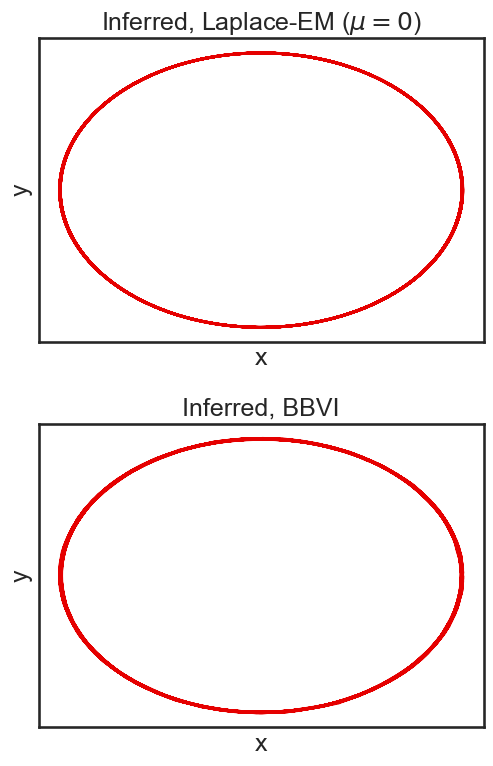
\includegraphics[width=\linewidth]{./Figures/vdp-good-mu0.png}
        \caption{}
        \label{goodvdp:b}
        \vspace{4ex}
    \end{subfigure}%%
    \begin{subfigure}[b]{0.33\linewidth}
        \centering
        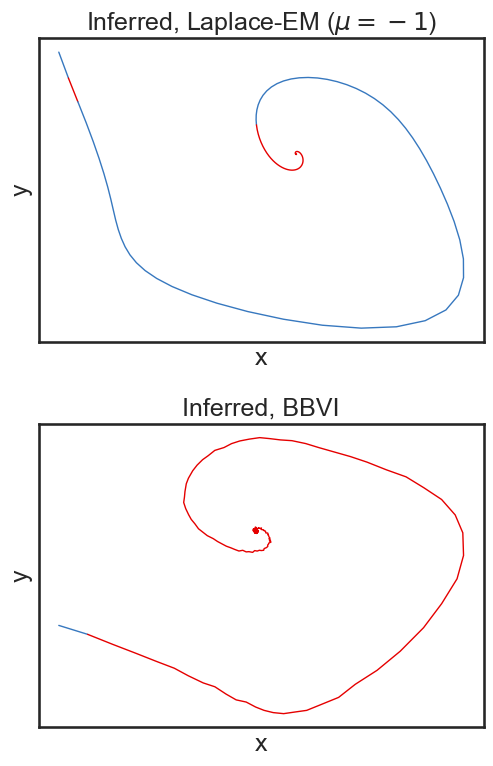
\includegraphics[width=\linewidth]{./Figures/vdp-good-mu-1.png}
        \caption{}
        \label{goodvdp:c}
        \vspace{4ex}
    \end{subfigure}
    \caption{Recovered trajectories of the Van der Pol oscillator from rSLDS model using the Laplace-EM and BBVI methods with a low amount of Gaussian noise present. In (A), $\mu = 1$ and while both methods accurately recover the true trajectories, Laplace-EM places the latent states with higher accuracy. In (B), $\mu = 0$ and the same results occur as in (A). While from the graph it is not evident, BBVI fails to place the latent states accurately and rather overlaps them. In (C), $\mu = -1$ and both methods fail to recover the latent states that are insightful.}
    \label{goodvdp}
\end{figure}



For the work of the paper, we will consider $\dot{y}$ to be the normal form of the Bautin bifurcation and observe how the system handles the three following behaviors around the bifurcation point. When $\beta_1,\beta_2 < 0$, the origin is stable with an unstable limit cycle around it. When $\beta_1,\beta_2 > 0$, the fixed point becomes stable and the limit cycle around unstable. In the specific subregion of $-1/4 \beta_2^2 < \beta_1 < 0$ and $\beta_2>0$, a second limit cycle emerges around the stable fixed point. The outer limit cycle is stable while the inner limit cycle is unstable. We demonstrate this behavior in Figure \ref{bautin-true}. On the left, $\beta_1 = \beta_2 < 0$ and the trajectory spirals into the stable fixed point and away from the unstable limit cycle. In the middle $\beta_1 = \beta_2 > 0$ and the trajectory travels to the stable limit cycle away from the unstable fixed point. On the right, $\beta_1 = -1/4 \beta_2^2$ and $\beta_2 > 0$ and we see the trajectory spiraling away from the unstable limit cycle into the stable limit cycle. 

To fit the Bautin system to the rSLDS model, we follow the same procedure as outlined for the Van der Pol. We will once again use an ODE solver on $\dot{y}$ for a fixed initial condition $(y_1,y_2) = (0,0.55)$ and $t\in[0,1000]$ using 10000 observations to create the sample data for the model. We used parameter values $(\beta_1,\beta_2) \in \left\{(-0.1,-0.1),(0.2,0.2),\left(-1/2,\sqrt{2}\right)\right\}$ which are near the Bautin bifurcation to get the true trajectories seen in Figure \ref{bautin-true}. Note that once again, the amount of noise added to the system is reduced to help the rSLDS model rediscover the dynamics. Fitting the rSLDS model using BBVI and Laplace EM, both methods recover the dynamics near the bifurcation point up to an affine transformation as seen in Figure \ref{bautinresults}. When $(\beta_1,\beta_2) = (-0.1,-0.1)$, both methods capture the dynamics of the stable fixed point although the BBVI results are less smooth. When $(\beta_1,\beta_2) = (0.2,0.2)$, both methods recover the stable limit cycle. Finally, when $(\beta_1,\beta_2) = (-1/2,\sqrt{2})$, both methods show the presence of an unstable limit cycle within a stable limit cycle. In each of the cases, both the Laplace EM and BBVI methods struggled to place two latent spaces and so we omitted the colors of the different states from the figure.  
\begin{figure}
    \centering
    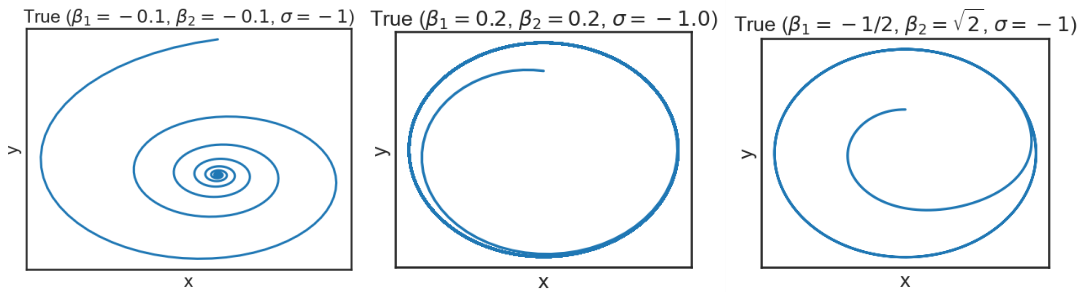
\includegraphics[width=0.9\textwidth,height=\textwidth,keepaspectratio]{./Figures/bautin-true.png}
    \caption{True trajectories of the Bautin system used to fit rSLDS model over $T\in[0,1000]$ with $1000$ observations. The initial condition of $(0,0.55)$ and $\sigma = -1$ is used for each trajectory. On the left, $\beta_1 = \beta_2 = -0.1$ and the trajectory spirals into the stable fixed point away from the unstable limit cycle. In the middle, $\beta_1 = \beta_2 = 0.2$ and the trajectory moves away from the unstable fixed point and into the stable limit cycle. On the right $\beta_1 = -1/2$ and $\beta_2 = \sqrt{2}$ and the trajectory spirals away from the unstable limit cycle on the inside and towards the stable limit cycle on the outside. }
    \label{bautin-true}
\end{figure}


\subsection{Remarks}
For both the methods, Laplace EM and BBVI, of the rSLDS model, the model accurately rediscovers the local dynamics near and on the bifurcation point but struggles to place two latent states in meaningful positions. More specially, fitting the model to the Van der Pol oscillator near the Hopf bifurcation highlights how the Laplace EM method outperforms the BBVI method at smoothly recreating the dynamics of the trajectory. Here the Laplace EM method is also able to place meaningful latent states for two of the cases near the bifurcation. Fitting the model to the Bautin system once again shows that the Laplace method outperforms the BBVI. Nevertheless, in both situations, the rSLDS model is only able to fit the dynamics of the model accurately when there is a low amount of noise present in the observation data.

\begin{figure}
    \begin{subfigure}[b]{0.333\linewidth}
        \centering
        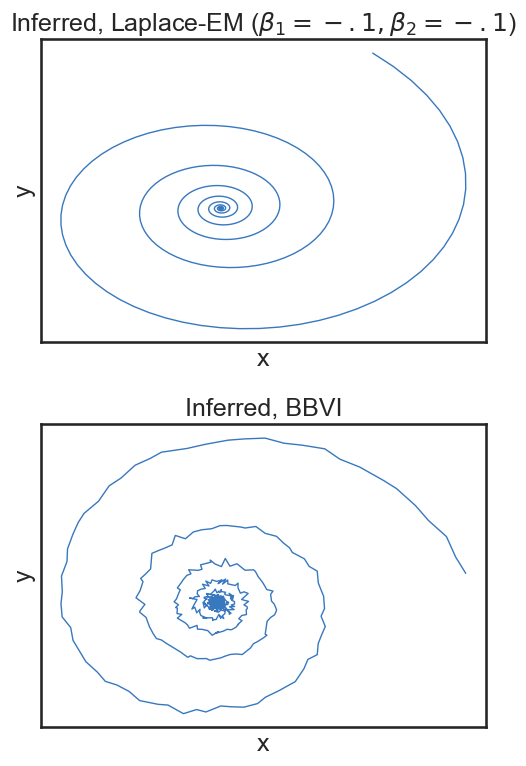
\includegraphics[width=\linewidth]{./Figures/bautin-stable.png}
        \caption{}
        \label{bautinresults:a}
        \vspace{4ex}
    \end{subfigure}%%
    \begin{subfigure}[b]{0.309\linewidth}
        \centering
        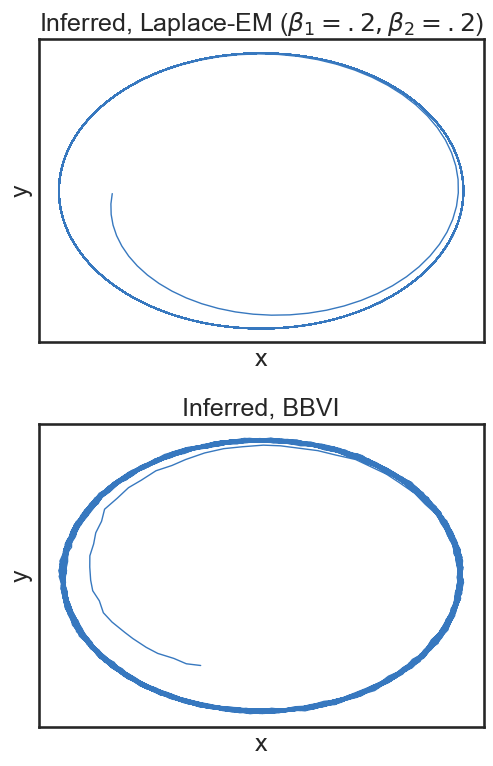
\includegraphics[width=\linewidth]{./Figures/bautin-unstab.png}
        \caption{}
        \label{bautinresults:b}
        \vspace{4ex}
    \end{subfigure}%%
    \begin{subfigure}[b]{0.33\linewidth}
        \centering
        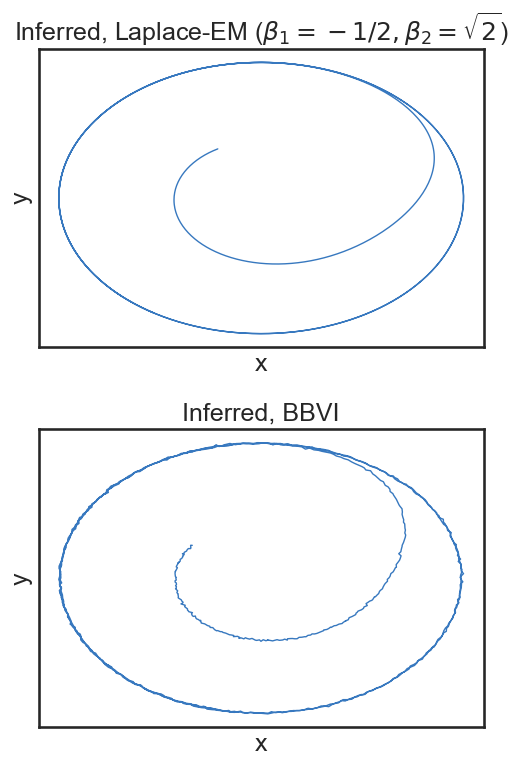
\includegraphics[width=\linewidth]{./Figures/bautin-lpc.png}
        \caption{}
        \label{bautinresults:c}
        \vspace{4ex}
    \end{subfigure}
    \caption{Recovered trajectories of the Bautin system from the rSLDS model using the Laplace-EM and BBVI methods with a low amount of Gaussian noise present. In (A), $\beta_1 = \beta_2 = -0.1$ and the Laplace-EM method smoothly recovers the true trajectory while the BBVI recovers a trajectory with noise. In (B), $\beta_1 = \beta_2 = 0.2$ and both methods perform similarly to (A). Note that once again it can be seen that the BBVI has more noise due to the variance (thickness of the line) of the limit cycle. In (C) $\beta_1 = -1/2$ and $\beta_2 = \sqrt{2}$ and the same results from (A) and (B) occur.}
    \label{bautinresults}
\end{figure}